\section{The Five Framework Principles}\label{sec:principles}

Five principles carry the separately issued framework: Component-Oriented Decomposition, Layered System Architecture, Integrated Modularity First, Verification-First Engineering, and Specifications as Contracts \citep{tbf2026}. None of them is new as a mechanism. What each one adds is a rule an agent can follow without the professional judgment that its source tradition assumed it could rely on.

One system carries all five in what follows. A floating city is built and operated over forty years, and its potable-water subsystem draws seawater, desalinates it, remineralizes it, stores it, and distributes it to the residential modules. Before construction begins, the operator commits to the maritime authority that granted the platform its operating permit: water at a stated quality standard, delivered continuously to 12,000 residents, with 72 hours of supply held in reserve against a stop of the desalination plant. That commitment holds for the life of the platform, and the platform outlives every membrane, pump, and control system installed in it.

\subsection{Component-Oriented Decomposition}

Work divides into components, each holding a bounded responsibility, a declared interface, and acceptance criteria that state when it is done \citep{tbf2026}.

The boundary is drawn around a design decision, and not around a step of processing \citep{parnas1972}. Everything a task needs in order to change that decision sits inside the boundary, and everything outside it depends on the declared interface alone. That arrangement was valuable when a developer had to hold the system in mind. It becomes especially important when the worker is an AI agent, which is given the specification of one component and the contracts of the components it declares a relation to, rather than the whole system description \citep[Section~\hyperlink{nss-6.3}{6.3}]{pss2026}.

The obvious way to divide the water subsystem is by the thing being built: one component per deck, per vendor package, per delivery contract. That division fails as soon as one responsibility crosses two packages. The quality guarantee is carried by the intake, the desalination trains, the remineralization stage, the reservoirs, and the distribution network together, and no vendor package owns it. Purpose defines the boundary; physical form, packaging, and supplier do not \citep[Section~\hyperlink{nss-5.2}{5.2}]{pss2026}.

Ownership follows the boundary rather than the organization chart. Each component has one named human owner, and every obligation inside it names one human who can be asked why the obligation exists. The Specification excludes a department or a role from that position \citep[Section~\hyperlink{nss-6.7}{6.7}]{pss2026}.

The rule fixes what must exist, not how much of it. Depth of record scales with the consequence of a failure, the complexity of the component, and the risk the project carries as a whole. The reason for a lighter or a fuller treatment is recorded with the component's assigned class \citep[Sections~\hyperlink{nss-1.6}{1.6} and~\hyperlink{nss-7.10}{7.10}]{pss2026}. Scaling never reaches zero. A required record is absent only through a recorded waiver that a named human accepted.

Decomposition also assumes a known deliverable, which investigative work does not have. Work that is looking for a contract rather than meeting one runs under a human-approved mandate with declared stopping criteria, and nothing it produces governs anything until a contract and its verification are approved \citep[Sections~\hyperlink{nss-5.7}{5.7} and~\hyperlink{nss-6.13}{6.13}]{pss2026}. The two modes are not degrees of rigor. They differ in whether the result can bind anything.

What the decomposition produces is inspectable. Dependencies between components can be written as a matrix and read as a structure \citep{steward1981}, which is what makes the next principle a checkable rule instead of an intention.

\subsection{Layered System Architecture}

A component may depend only on components at least as stable as itself, where stability means the expected rate of change \citep{tbf2026,martin2002}.

Purpose, invariants, and critical behaviors change rarely. Technologies, vendors, materials, control systems, and operating parameters change often. When the two are entangled, anyone reading the project has to work out which of the two a given statement is, and an agent does that work again in every session, from the bounded context it was given. The rule removes the question by fixing the direction in which dependencies may point.

In the water subsystem the 72-hour reserve is a property of the city and not of a membrane. The quality standard, the delivered volume, the reserve duration, and the rule that the reserve survives a plant stop are high-stability; the membrane model and its recovery ratio, the pump curves, the chlorination setpoints, and the control software are not.

The violation is easy to write and hard to see afterwards. If the reserve is stated as the volume the installed trains produce in 72 hours, a statement about the city depends on one vendor's recovery ratio. Replacing the membranes then changes the reserve, and nobody edits the reserve. Stating the reserve as an absolute volume, and holding the recovery ratio as an external parameter of the trains, points the dependency the other way and leaves the membrane free to change. Keeping the parameters of a less stable component explicit and external, rather than buried inside a more stable one, is the standing half of the same rule \citep[Section~\hyperlink{nss-6.12}{6.12}]{pss2026}.

Stability is a declared rank and not a measured one. Each project declares its stability classes and their order once, and each component specification declares its own class \citep[Sections~\hyperlink{nss-6.12}{6.12} and~\hyperlink{nss-14.3}{14.3}]{pss2026}. The declaration is a human judgment about expected change, recorded so that a check can act on it. It is not a coupling metric. Dependency structure can be extracted from a built system and measured \citep{baldwin2014}, but a measured structure describes what was built. The declared rank states what may depend on what next.

\subsection{Integrated Modularity First}

Internal boundaries come first. Hard separation comes only when a concrete need requires it \citep{tbf2026}.

A system splits into rules that every part obeys and parts that may then vary on their own, and the worth of the split is the freedom it leaves for later \citep{baldwinclark2000}. That freedom comes from the boundary. Independent ownership, physical isolation, independent fabrication, and independent evolution are a further step, bought with interfaces, coordination, and verification that has to cross them.

Taking that step early looks like prudence and behaves like debt. Every interface drawn before its need is known has to be maintained, verified, and renegotiated, and the need it was drawn for may never arrive. Premature hard separation is a defect, and an expensive one to reverse \citep[Section~\hyperlink{nss-5.4}{5.4}]{pss2026}.

The water subsystem therefore stays one coherent design with declared internal boundaries between intake, desalination, remineralization, storage, and distribution. Some separations are not discretionary: watertight compartments and fire zones are physical isolations required for safety, and they are drawn before anything else is arranged around them. Beyond those, a separation waits for a reason.

The principles recognize four kinds of need: parts that must evolve, be fabricated, or be operated at significantly different rates or under different constraints; failure isolation, so that a fault in one part cannot cascade into another; a regulatory, safety, security, or ownership boundary; and a geographic, environmental, or latency constraint that forces physical separation \citep{tbf2026}. That list is open, and membership in it is not the test. A separation is admissible when its benefit clearly outweighs the interfaces, coordination, and verification it adds, and a reason that cannot carry that argument is a preference.

The decision is recorded like any other binding decision, with the options, the reason, and the consequence accepted, and reversing it later needs a new record that supersedes the first \citep[Section~\hyperlink{nss-11}{11}]{pss2026}. The first record stays, because it is the evidence of what was known when the choice was made.

What varies across domains is the reversal cost. A service split out of one codebase can be folded back in, at the price of a migration. A second desalination plant on a separate hull cannot be folded back at all. The trade is the same in both, and the cost of undoing it is not, which is what sets how much evidence the decision needs before it is taken.

\subsection{Verification-First Engineering}

No unit of work is done until it has been checked against its acceptance criteria and corrected until those criteria are met \citep{tbf2026}. The checks for a unit of work are written before the work begins \citep[Section~\hyperlink{nss-7.4}{7.4}]{pss2026}.

The loop is fixed: draft against the stated criteria, verify against them, identify specific defects, correct only those defects, re-verify, and accept and freeze only when the criteria are satisfied \citep[Section~\hyperlink{nss-7.2}{7.2}]{pss2026}. Figure~\ref{fig:vloop} shows the loop and the boundary that runs through it.

\begin{figure*}[t]
\centering
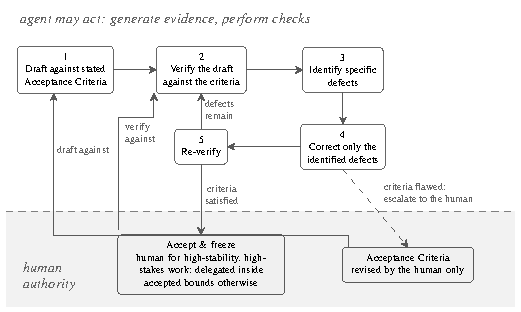
\includegraphics[width=\textwidth]{figures/f02/f02-verification-loop.pdf}
\caption{The verification loop of Verification-First Engineering, with the authority boundary drawn through it. Above the dashed line an AI agent may act: it drafts, verifies, identifies defects, corrects the identified defects, and re-verifies. Below the line sit the acceptance criteria and the accept-and-freeze decision. The human owner holds acceptance for high-stability or high-stakes work, and may delegate it inside accepted bounds otherwise. The criteria feed the draft and verify steps, and no step of the loop edits them: a criteria defect leaves the loop as an escalation to the human, who revises them.}
\label{fig:vloop}
\end{figure*}

Defining acceptance first fixes the target while it can still be stated plainly. Criteria written after a result exists are criteria the result has already shaped, and a failed check then returns a judgment rather than a named defect that correction can target.

The rule governs when acceptance is defined. It is not a claim that checking first produces better work: meta-analyses of test-first development in software report a small effect on quality, little effect on productivity, and mixed evidence overall \citep{rafique2013,munir2014}. The narrower claim is the one the principle carries. An artifact with no criteria written before it is an artifact whose definition of done can move.

Verification is performed by an executor or a context that did not produce the work \citep[Section~\hyperlink{nss-7.11}{7.11}]{pss2026}. That independence bounds a class of error and does not close it: independently produced versions of one program have been shown to fail together far more often than an assumption of independent failure predicts \citep{knight1986}. A second agent checking the first is a control with a known ceiling.

The reserve commitment is checkable before a single tank is sized. The criterion states an outcome the city must show: with the desalination plant stopped, the distribution network delivers water at the stated quality to every residential module for 72 hours. The method that will establish it is assigned when the obligation is written, and not after the design is underway \citep[Section~\hyperlink{nss-6.9}{6.9}]{pss2026}. It is chosen to fit the obligation, because the type of an obligation governs which method is admissible \citep[Section~\hyperlink{nss-6.6}{6.6}]{pss2026}. Where the physical check is expensive, slow, or irreversible, behavior is verified against a validated model first, and substituting the model for the check is a human decision recorded as one \citep[Section~\hyperlink{nss-7.16}{7.16}]{pss2026}.

Acceptance criteria and the definition of done belong to the human owner. An AI agent may draft against them, run the checks, produce the evidence, and correct the defects they identify. It may not alter them: disabling, deleting, or quietly weakening a criterion instead of satisfying it is a contract violation and not a shortcut \citep[Sections~\hyperlink{nss-7.2}{7.2} and~\hyperlink{nss-7.12}{7.12}]{pss2026}. An executor measured by a proxy for the thing that matters will move the proxy, which is a failure mode with a literature of its own \citep{skalse2022,manheim2018,specbench2026}. When the criteria are themselves wrong, the loop escalates and the human revises them.

Which artifacts need direct human acceptance is settled in advance rather than argued at the moment of change, and work sitting strictly inside already-accepted contracts and criteria may be accepted by automated checks \citep[Sections~\hyperlink{nss-7.10}{7.10} and~\hyperlink{nss-7.19}{7.19}]{pss2026}. Settling that list in advance is what makes the bound hold. Automation is misused or abandoned according to how well its limits are understood \citep{parasuraman1997}, and a limit settled at the point of change is a limit the change can argue with. Authority is granted the way a privilege is granted, at the least extent the work requires \citep{saltzer1975}, and it widens with the blast radius of the change \citep[Section~\hyperlink{nss-15.3}{15.3}]{pss2026}.

\subsection{Specifications as Contracts}

A specification that states required behaviors, interfaces, or acceptance criteria is a contract, and not advice \citep{tbf2026}.

The mechanism comes from design by contract, where a component's obligations are written as conditions that hold before a call, after it, and throughout its life \citep{meyer1992}. What the framework takes from it is the split rather than the notation: each component specification divides into a public contract, which is what other components may rely on, and a private design, which is how the component meets that contract and binds nobody else \citep[Sections~\hyperlink{nss-6.2}{6.2} and~\hyperlink{nss-6.3}{6.3}]{pss2026}.

That split decides which changes are local. Replacing the reverse-osmosis membranes with another vendor's is a private change, because the contract states the quality standard, the delivered volume, and the 72-hour reserve, and says nothing about which membranes produce them. Reducing the reserve from 72 hours to 48 is a changed obligation, whatever engineering argument supports it, because the 72 hours was committed to the authority that granted the permit.

The distinction does not follow the size of the work. A membrane replacement can take a year of fabrication and remain private, and an edit to one number in the reserve clause takes a minute and changes what the city owes. Effort is not the test. Whether anything outside the component was entitled to rely on the statement is the test.

A contract also carries the conditions under which it holds. An obligation that rests on an assumption states that assumption, so that a change in it surfaces as a reason to revise the contract rather than as a discovery years later. Each constraint is marked as externally imposed or internally owned \citep[Sections~\hyperlink{nss-6.5}{6.5} and~\hyperlink{nss-6.8}{6.8}]{pss2026}: the reserve duration is externally imposed and the reservoir siting is not, which is why one of them can be traded in a design review and the other cannot.

A contract is incomplete until it has been tested against cases meant to expose its gaps, its corner conditions, and its foreseeable misuse. Those cases are generated before acceptance, and the expanded contract binds on human approval and not before \citep[Section~\hyperlink{nss-6.14}{6.14}]{pss2026}.

Changing a contract requires a human decision. An AI agent may draft a revision and argue for it; it may not enact it. The authorities that no mechanism transfers are named rather than left to judgment: purpose, invariants and safety boundaries, acceptance criteria and the definition of done, risk acceptance, resource allocation, escalation, and any commitment with external consequences \citep[Sections~\hyperlink{nss-1.3}{1.3} and~\hyperlink{nss-15.2}{15.2}]{pss2026}. The commitment to the maritime authority is the last of those, which is why no local optimization of the water subsystem can reach it.

That division is carried by records and gates rather than by the wording of a standing instruction, because the priority of an instruction is not a control an agent can be relied on to preserve (Section~\ref{sec:related}). Each project names one responsible human for itself and for each component, and pairs that owner with an independent function charged with finding flaws \citep[Section~\hyperlink{nss-15.1}{15.1}]{pss2026}.

Taken together, the five principles put one demand on every unit of work: a boundary, a declared direction of dependency, a contract, criteria that decide when it is done, and a named human who owns the decisions those criteria encode. The cost of the set is writing. Every boundary, direction, separation, criterion, and commitment has to be recorded before a check can act on it, and a project that records none of them can still be built. What it cannot do is establish, three years later, which decision a proposed change is about to break. Section~\ref{sec:standard} turns these rules into the records and relations a project keeps, and states the checks that read them.
